\documentclass{beamer}
\usepackage[utf8x]{inputenc}
\usepackage{amssymb}
\usepackage{tikz}
\usetikzlibrary{automata, positioning, chains,fit,shapes}
\usepackage{color}
\definecolor{keywordcolor}{rgb}{0.7, 0.1, 0.1}   % red
\definecolor{commentcolor}{rgb}{0.4, 0.4, 0.4}   % grey
\definecolor{symbolcolor}{rgb}{0.0, 0.1, 0.6}    % blue
\definecolor{sortcolor}{rgb}{0.1, 0.5, 0.1}      % green
\usetheme{Dresden}
\usepackage{listings}
\def\lstlanguagefiles{lstlean.tex}
\lstset{
    language=lean,
}
\setbeamercolor{block body alerted}{bg=alerted text.fg!10}
\setbeamercolor{block title alerted}{bg=alerted text.fg!20}
\setbeamercolor{block body}{bg=structure!10}
\setbeamercolor{block title}{bg=structure!20}
\setbeamercolor{block body example}{bg=green!10}
\setbeamercolor{block title example}{bg=green!20}

\title[Finite sets]{Formalization of finite sets in Lean}
\author[J. Tantow]{Johannes Tantow}
\addtobeamertemplate{navigation symbols}{}{%
    \usebeamerfont{footline}%
    \usebeamercolor[fg]{footline}%
    \hspace{1em}%
    \insertframenumber/\inserttotalframenumber
}
\begin{document}
    \maketitle
    \begin{frame}[fragile]{\textbf{Formalization} of finite sets \textbf{in Lean}}
        \includegraphics[width=1\textwidth]{Lean_Preview.png}
    \end{frame}

    \begin{frame}{Formalization of finite \textbf{sets} in Lean}
        \begin{block}{Naive set theory}
            A set is 
        \end{block}
        \begin{block}{Zermelo-Fraenkel set theory:}
        \begin{enumerate}
            \item Axiom of Extensionality:
            $\forall x, y.(\forall z. (z \in x \leftrightarrow z \in y) \rightarrow x=y)$
            
            \item Axiom of Regularity 
            $\forall x. (x \neq \emptyset \rightarrow \exists y. y \in x \land y \cap x = \emptyset ) $
            
            \item Axiom of Empty Set: $\exists y. \forall x: \neg x \in y$
            \item ...
            
        \end{enumerate}
        \end{block}
        \pause
        \begin{block}{Lean}
        $(s: \text{{set}}\ A) = A \to \text{{Prop}}$
        \end{block}
    \end{frame}
    \begin{frame}{Formalization of \textbf{finite sets} in Lean}
        \begin{enumerate}[<+->]
            \item there is a list containing all elements
            \item there is a tree containing all elements
            \item there exists some $N \in \mathbb{N}$ such that every list of length at least $N$ contains duplicates
            \item there is no surjection from this set to the natural numbers
            \item ...
        \end{enumerate}
    \end{frame}
    \begin{frame}[fragile]{Finite sets in automata theory}
        \begin{minipage}{0.30\linewidth}
            \centering
            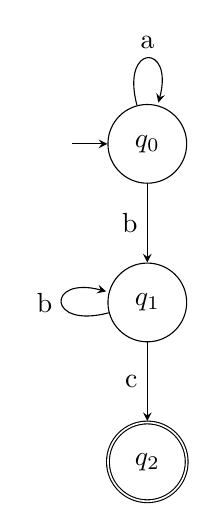
\begin{tikzpicture}[
                ->,
                >=stealth,
                node distance=1cm,
                every state/.style={draw, circle, minimum size=1cm},
                initial text={}
              ]
              
              % States
              \node[state, initial] (q0) {$q_0$};
              \node[state, below=of q0] (q1) {$q_1$};
              \node[state, accepting, below=of q1] (q2) {$q_2$};
              
              % Transitions
              \draw (q0) edge[loop above] node[above] {a} ();
              \draw (q0) edge[left] node {b} (q1);
              \draw (q1) edge[loop left] node[left] {b} ();
              \draw (q1) edge[left] node {c} (q2);
              \end{tikzpicture}
            
            $(\mathbf{Q}, s ,\mathbf{\Sigma}, F, \delta)$
            \end{minipage}
            \hfill
            \begin{minipage}{0.65\linewidth}
            \centering
            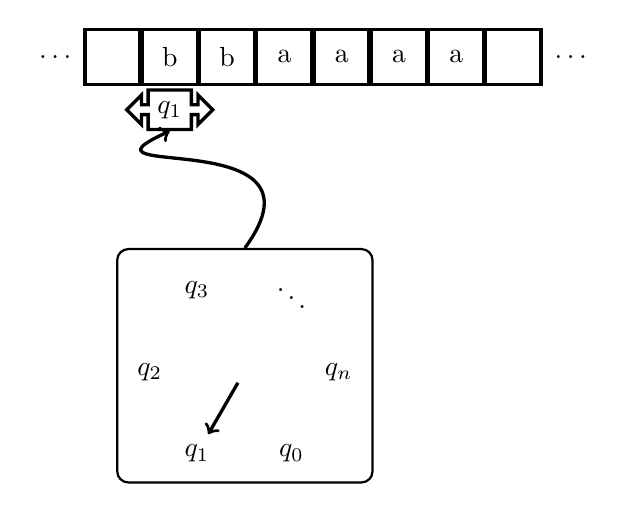
\begin{tikzpicture}[scale={0.8}]
                \tikzstyle{every path}=[very thick]
                
                \edef\sizetape{0.7cm}
                \tikzstyle{tmtape}=[draw,minimum size=\sizetape]
                \tikzstyle{tmhead}=[arrow box,draw,minimum size=.5cm,arrow box
                arrows={east:.25cm, west:0.25cm}]
                
                %% Draw TM tape
                \begin{scope}[start chain=1 going right,node distance=-0.15mm]
                    \node [on chain=1,tmtape,draw=none] {$\ldots$};
                    \node [on chain=1,tmtape] {};
                    \node [on chain=1,tmtape] (input) {b};
                    \node [on chain=1,tmtape] {b};
                    \node [on chain=1,tmtape] {a};
                    \node [on chain=1,tmtape] {a};
                    \node [on chain=1,tmtape] {a};
                    \node [on chain=1,tmtape] {a};
                    \node [on chain=1,tmtape] {};
                    \node [on chain=1,tmtape,draw=none] {$\ldots$};
                \end{scope}
                
                %% Draw TM Finite Control
                \begin{scope}
                [shift={(3cm,-5cm)},start chain=circle placed {at=(-\tikzchaincount*60:1.5)}]
                \foreach \i in {q_0,q_1,q_2,q_3,\ddots,q_n}
                    \node [on chain] {$\i$};
                
                % Arrow to current state
                \node (center) {};
                \draw[->] (center) -- (circle-2);
                
                \node[rounded corners,draw=black,thick,fit=(circle-1) (circle-2) (circle-3) 
                      (circle-4) (circle-5) (circle-6),
                            ] (fsbox)
                        {};
                \end{scope}
                
                %% Draw TM head below (input) tape cell
                \node [tmhead,yshift=-.3cm] at (input.south) (head) {$q_1$};
                
                %% Link Finite Control with Head
                \path[->,draw] (fsbox.north) .. controls (4.5,-1) and (0,-2) .. node[right] 
                            (headlinetext)
                             {} 
                            (head.south);                
                \end{tikzpicture}
            
            $(\mathbf{Q}, \mathbf{\Sigma},\mathbf{\Gamma}, \delta, q_0,\textvisiblespace  ,\mathbf{F})$
            \end{minipage}
        
        
    \end{frame}
    \begin{frame}{Finite sets in databases}
        
    \end{frame}

    \begin{frame}[fragile]{Formalization of \textbf{finite sets in Lean} - so far}
        \begin{lstlisting}
structure finset (α : Type*) :=
    (val : multiset α)
    (nodup : nodup val)


section lattice
    variables (α : Type*) [decidable_eq α] 
    instance : has_union (finset α) 
    instance : has_inter (finset α)

    ...
        \end{lstlisting}
    \end{frame}
\begin{frame}{HIT from HoTT}
    
\end{frame}

\begin{frame}[fragile]{Size}
    \begin{lstlisting}[escapeinside={(*}{*)}]        
def size{A:Type}: KSet A -> A
| (*$\emptyset$ *) := 0
| {a} := 1
| (X ∪ Y) := (* \textcolor{red}{?}*)
    \end{lstlisting}
\pause
    \begin{block}{Proposal}
        $size(X \cup Y) := size(X) + size (Y) - size(X \cap Y)$
    \end{block}
\end{frame}

\begin{frame}[fragile]{Size problems}
    $\bigl( \{1\} \cup \{2\} \bigr) \cup \bigl( \{2\} \cup \{3\} \bigr) $



    $ \{1\} \cup \bigl( \{2\} \cup \bigl( \{2\} \cup \{3\} \bigr) \bigr) $
\pause
\begin{lstlisting}[escapeinside={(*}{*)}]
def to_list: Kuratowski A -> list A
| (*$\emptyset$ *) := nil
| {a} := a :: nil
| (X ∪ Y) := to_list X ++ to_list y

def size (X: Kuratowski A): (*$\mathbb{N}$*) := len(to_list(X))
\end{lstlisting}
\end{frame}
    
    \begin{frame}[fragile]{Axioms and Functions}
        \begin{lstlisting}[escapeinside={(*}{*)}]
axiom union_comm (X Y: KSet A): X ∪ Y = Y ∪ X

noncomputable def first{A:Type} [nonempty A]: KSet A -> A
| (*$\emptyset$ *) := classical.some A
| {a} := a
| (X ∪ Y) := first (X)
    \end{lstlisting}
        \begin{block}{}
            Axioms don't care about preservation by functions
        \end{block}
    \end{frame}
    \begin{frame}[fragile]{One million dollars}
        \begin{lstlisting}
theorem p_eq_np (l: language)(l_np: l ∈ NP):l ∈ P :=
begin
    exfalso,
    let X:= {1} ∪ {2},
    have first1: first (X) = 1,
    dunfold first,
    refl,
    have first2: ¬  first(X) = 1,
    have X2: X = {2} ∪ {1} by union_comm,
    rw X2,
    simp[first],
    exact absurd first1 first2,
end
            \end{lstlisting}
    \end{frame}
    \begin{frame}{Quotients}
        \begin{definition}
            Let $A: \text{{Type}}$ and $R: A \times A \to \text{{Prop}}$ be an equivalence relation.
            Then $A/R$, the quotient of $A$ by $R$, is a type.
        \end{definition}
    \pause
    Equivalence relations:
    \begin{enumerate}[<+->]
        \item $R(X,Y) := (X = Y) \lor (\exists V, W. X= (V \cup W) \land Y = (W \cup Y)) \lor ...$
        \item $R(X,Y) := \forall a. a \in X \leftrightarrow a \in Y$
    \end{enumerate}

    \end{frame}
    \begin{frame}{Lifting}
    
    \end{frame}
    \begin{frame}{Trees}
        
    \end{frame}
    \begin{frame}{Insertion}
        definition

        Semantics

        Order result
    \end{frame}
    \begin{frame}

    \end{frame}
    \begin{frame}[fragile]{Tree equality}
        \begin{figure}
            \begin{minipage}[t]{0.45\linewidth}
                \centering
                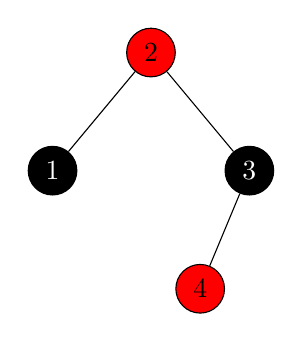
\begin{tikzpicture}[
                    red_node/.style={circle, draw=black, fill=red, minimum size=6mm},
                    black_node/.style={circle, draw=black, fill=black, text=white, minimum size=6mm},
                    level/.style={sibling distance=25mm/#1}
                ]
                    \node[red_node] {2}
                        child {
                            node[black_node] {1}
                        }
                        child {
                            node[black_node] {3}
                                child {
                                    node[red_node] {4}
                                }
                                child[missing] {}
                        };
                \end{tikzpicture}
                \caption{flatten T = [1,2,3,4]}
            \end{minipage}\hfill
            \begin{minipage}[t]{0.45\linewidth}
                \centering
                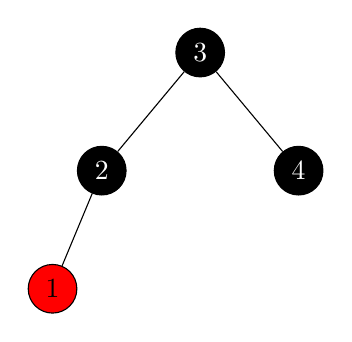
\begin{tikzpicture}[
                    red_node/.style={circle, draw=black, fill=red, minimum size=6mm},
                    black_node/.style={circle, draw=black, fill=black, text=white, minimum size=6mm},
                    level/.style={sibling distance=25mm/#1}
                ]
                    \node[black_node] {3}
                        child {
                            node[black_node] {2}
                                child {
                                    node[red_node] {1}
                                }
                                child[missing] {}
                        }
                        child {
                            node[black_node] {4}
                        };
                \end{tikzpicture}
                \caption{flatten T = [1,2,3,4]}
            \end{minipage}

            Use a quotient based on flatten.
        \end{figure}
    \end{frame}

    \begin{frame}{Properties of flatten}
        \begin{block}{Lemma(Extensionality)}
            $flatten (T1) = flatten (T2) \leftrightarrow \forall x, x \in T1 \leftrightarrow x \in T2$
        \end{block}
        \begin{block}{Proof}
            Idea:
                \begin{itemize}
                    \item two list are equal iff they are both sorted and permutations of each other
                    \item Ordered trees are sorted
                    \item Ordered trees are duplicate free: permutations
                \end{itemize}
        \end{block}
        \begin{block}{Lemma}
            size(T) = len(flatten(T))
        \end{block}
    \end{frame}

    \begin{frame}[fragile]{Induction on trees}
        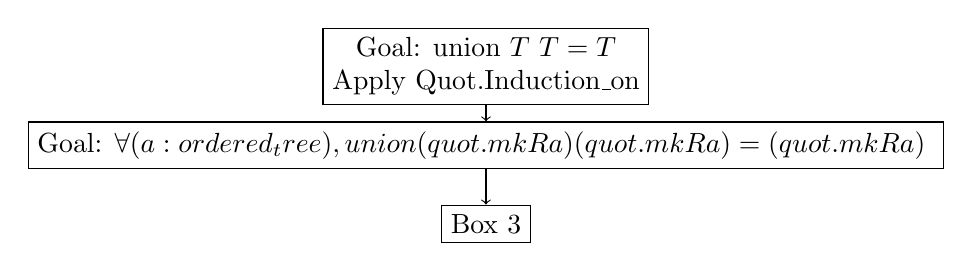
\begin{tikzpicture}
            \node [draw, rectangle, align=center] (box1) {Goal: union $T$ $T = T$\\ Apply Quot.Induction\_on};
            \node [draw, rectangle, below of=box1, align=center] (box2) {Goal: $\forall (a: ordered_tree),  union (quot.mk R a) (quot.mk R a) = (quot.mk R a)$  };
            \node [draw, rectangle, below of=box2, align=center] (box3) {Box 3};
            
            \draw [->] (box1) -- (box2);
            \draw [->] (box2) -- (box3);
          \end{tikzpicture}
    \end{frame}
    

    \begin{frame}[fragile]{Don't repeat yourself}
        Mathlib data.set
        \begin{lstlisting}
theorem mem_inter_iff (x : α) (a b : set α) :
    x ∈ a ∩ b ↔ (x ∈ a ∧ x ∈ b)
        \end{lstlisting}
        Kuratowski sets
        \begin{lstlisting}
lemma in_intersection_iff_in_both (X Y: Kuratowski A) (a:A): a ∈ (X ∩ Y) =  (a ∈ X ∧ a ∈ Y)
        \end{lstlisting}

    \end{frame}
    \begin{frame}{Finite by proof}
        \begin{definition}
            A finite set $S_f$ is a pair of a set $S$ and a proof of its finiteness.
        \end{definition}
        \pause
        Examples
        \begin{enumerate}
            \item Bijection finite: $\exists (n:\mathbb{N}), (f: \mathbb{N} \to A).\; \text{{set.bij\_on}}\; f \;\{ x \in \mathbb{N} \mid x < n\} \;S$
            \item Surjection finite: $\exists (n:\mathbb{N}), (f: \mathbb{N} \to A).\; \text{{set.surj\_on}}\; f \;\{ x \in \mathbb{N} \mid x < n\} \;S $
            \item Dedekind finite: $\forall (S' \subsetneq S), (f: A \to A).\; \neg \text{{set.bij\_on}}\; f\; S'\; S$
        \end{enumerate}
    \end{frame}
    \begin{frame}[fragile]{Simple sets}
        \begin{lemma}
            $ \varnothing $ is finite.
        \end{lemma}
        $f: n \mapsto classical.some$ $A$
        \begin{lemma}
            For all $a:A$, $\{ a\}$ is finite.
        \end{lemma}
        $f: n \mapsto a$
        \begin{block}{Type Requirement}
        A has to be nonempty
        \end{block}
    \end{frame}

    \begin{frame}[fragile]{Size}
\begin{lstlisting}
def is_finite {A: Type} (S: set A): Prop := 
    ∃ (n:ℕ) (f: ℕ → A), 
    set.bij_on f (set_of (λ (a:ℕ), a < n)) S
\end{lstlisting}

How to get $n$ for $\exists n, \phi(n)$ ?
\begin{enumerate}
    \item classical.choie: Uses AC
    \item nat.find if $\phi$ is decidable
\end{enumerate}

    \begin{lstlisting}
noncomputable def size (s: set A) (fin: is_finite s): ℕ
:= classical.some fin
\end{lstlisting}
    \end{frame}

    \begin{frame}{Noncomputable size}
        \begin{itemize}
            \item Let $M$ be a Turing-machine.
            \item Then $\{M\}$ is a finite set.
            \item There exists a $FO$ formula $\phi(M)$, that is true whenever a TM stops on the empty input
            \item Then $\{ M' \mid \phi (M') \land M' \in \{M\}\}? $ is finite.
            \item What is the size of $\{ M' \mid \phi (M') \land M' \in \{M\}\}? $
        \end{itemize}
    \end{frame}

    \begin{frame}[fragile]{Computable size}
\begin{lstlisting}
def set_size: listSet A -> ℕ
| nil := 0
| (hd::tl) := if hd ∈ tl then set_size(tl) else set_size(tl) + 1
\end{lstlisting}
\begin{lstlisting}
def singleton: A -> listSet A := {a}
def comprehension: (A -> bool) -> listSet A -> listSet A
\end{lstlisting}
\begin{block}{Lean detail}
    Every function $A \to bool$ is computable, whereas $A \to Prop$ is not.
\end{block}


\begin{lstlisting}
noncomputable def comprehension': (A -> Prop) -> listSet A -> listSet A
\end{lstlisting}
\end{frame}

\begin{frame}[fragile]{Overview of finite sets}
    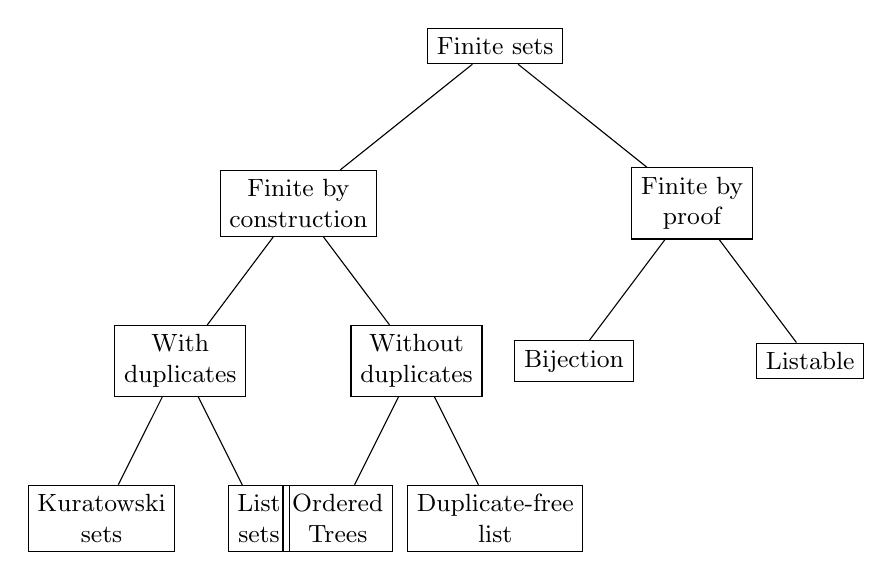
\begin{tikzpicture}[
        every node/.style={rectangle, draw, align=center, font=\small},
        level 1/.style={sibling distance=50mm},
        level 2/.style={sibling distance=30mm},
        level 3/.style={sibling distance=20mm},
        level 4/.style={sibling distance=10mm},
        level distance=20mm
      ]
      \node {Finite sets}
        child {node {Finite by\\ construction}
          child {node {With \\ duplicates}
            child {node {Kuratowski\\ sets}}
            child {node {List\\ sets}}
            }
          child {node {Without\\ duplicates}
            child {node {Ordered\\ Trees}}
            child {node {Duplicate-free\\ list}}
          }
        }
        child {node {Finite by\\ proof}
          child {node {Bijection}}
          child {node {Listable}}
        };
      \end{tikzpicture}
\end{frame}
\begin{frame}
    
\end{frame}
\end{document}
